\documentclass[11pt,letterpaper]{article}

\usepackage{graphicx}
\usepackage{geometry}
\usepackage{amsmath}
\usepackage{amssymb}
\usepackage{booktabs}
\usepackage{xcolor}
\usepackage{listings}
\usepackage{url}
\usepackage{hyperref}
\usepackage{natbib}

\geometry{margin=1in}
\hypersetup{colorlinks=true, linkcolor=black, citecolor=black, urlcolor=blue}

\title{\textbf{Beam Recall as the Binding Constraint: An Empirical Study of World-Probing for Annotation-Free NL-to-FOL Candidate Selection}}

\author{
AMGrobelnik \\
\textit{AI Inventor} \\
\href{https://github.com/AMGrobelnik/ai-invention-8ad782-beam-recall-as-the-binding-constraint-an}{github.com/AMGrobelnik/ai-invention-8ad782-beam-recall}
}

\date{}

\begin{document}

\maketitle

\begin{abstract}
Converting natural language (NL) to first-order logic (FOL) is foundational for neuro-symbolic reasoning, yet selecting the semantically faithful translation from a beam of candidates remains unsolved at test time. We propose \textbf{Heterogeneous-Oracle World-Probing (HOWP)}, an annotation-free candidate-selection pipeline that generates minimal named-domain world models, evaluates each FOL candidate deterministically against those worlds, and scores candidates by cross-world agreement with an independent LLM oracle. We conduct a two-regime empirical study to characterize when HOWP can succeed. On FOLIO (204 validation examples, Llama-3.1-8B generator, $k{=}5$ beam), beam recall is only 38\%, and all seven selection conditions---including HOWP, top-1 generation, self-consistency, and three ablations---are statistically indistinguishable (all BH-corrected McNemar $p > 0.77$; effect sizes Cohen's $h \leq 0.14$). Nevertheless, the cross-world agreement score retains a statistically significant discriminative signal (AUC-ROC $= 0.660$, Kendall $\tau = 0.212$, $p = 0.0009$), confirming that the mechanism is sound but cannot overcome the beam recall ceiling. On a synthetic single-premise benchmark with Llama-3.1-70B (beam recall $= 100\%$), direct LLM oracle judgment achieves 99\% accuracy---outperforming HOWP (93\%), top-1 (94\%), and self-consistency (94\%)---because oracle noise (66.7\% in-distribution accuracy) introduces errors precisely when the world-probing scaffold is unnecessary for simple predicate-application sentences. Contrary to ensemble-theory motivation, the same-model oracle numerically exceeds the heterogeneous oracle on FOLIO (24.5\% vs.\ 20.6\%, $p = 0.77$), indicating that syntax calibration between generator and oracle outweighs parametric independence at 7B parameter scale. These results establish beam recall as the primary bottleneck for world-probing selection methods and chart a precise roadmap for when the HOWP mechanism can add value.
\end{abstract}

%% ============================================================
\section{Introduction}
%% ============================================================

Converting natural language (NL) into first-order logic (FOL) is a foundational step in neuro-symbolic reasoning pipelines \citep{Olausson2023, Pan2023, Wei2022}. Given a set of NL premises and a conclusion, a downstream Z3 solver can determine entailment, contradiction, or neutral relationships---but only if the FOL translations faithfully capture the meaning of the original sentences. The NL-to-FOL translation problem thus has two separable components: \emph{syntactic validity} (is the formula well-formed?) and \emph{semantic faithfulness} (does it mean the same thing as the NL sentence?).

Recent generation methods have addressed syntactic validity substantially. NL2LOGIC \citep{Putra2025} achieves 99\% syntactic accuracy via abstract syntax tree (AST)-guided generation, and Grammar-Constrained Decoding (GCD) \citep{Geng2023} enforces syntactic validity at the token level. Yet neither approach provides a \emph{test-time} mechanism for selecting among semantically distinct syntactically-valid candidates. Modern LLMs typically generate multiple plausible translations for any NL sentence in a $k$-candidate beam, and the beam often contains both correct and incorrect formulations that cannot be distinguished by syntactic checks alone.

\citet{Brunello2026} (AAAI 2026) independently identify a related gap: the widely-used Logical Equivalence score treats FOL formulas propositionally, assigning fixed truth values regardless of domain elements. Their model-theoretic correction requires gold FOL annotations, making it a benchmarking tool rather than a test-time selection mechanism. No existing work provides annotation-free, per-candidate faithfulness scoring at inference time.

We propose \textbf{Heterogeneous-Oracle World-Probing (HOWP)}: generate diverse minimal world models over named domains, evaluate each candidate's truth profile deterministically, and score by cross-world agreement with an independent LLM oracle from a different training lineage than the generator. The heterogeneity is motivated by ensemble theory \citep{Breiman2001, Lakshminarayanan2017}: parametric independence should ensure that oracle-formula disagreements reflect genuine semantic mismatch rather than shared intra-model bias.

We evaluate HOWP in two regimes chosen to isolate the variables that govern its effectiveness. The first regime (FOLIO, 204 examples, Llama-3.1-8B generator \citep{Dubey2024}) yields a beam recall of only 38\%, creating a hard ceiling on any selection strategy. The second regime (synthetic single-premise benchmark, 100 examples, Llama-3.1-70B generator) achieves 100\% beam recall, removing the ceiling and revealing whether the world-probing mechanism itself adds value once candidates are available. Across both regimes, we apply full statistical testing---bootstrap confidence intervals and BH-corrected McNemar's tests on all pairwise comparisons.

\begin{figure*}[!t]
  \centering
  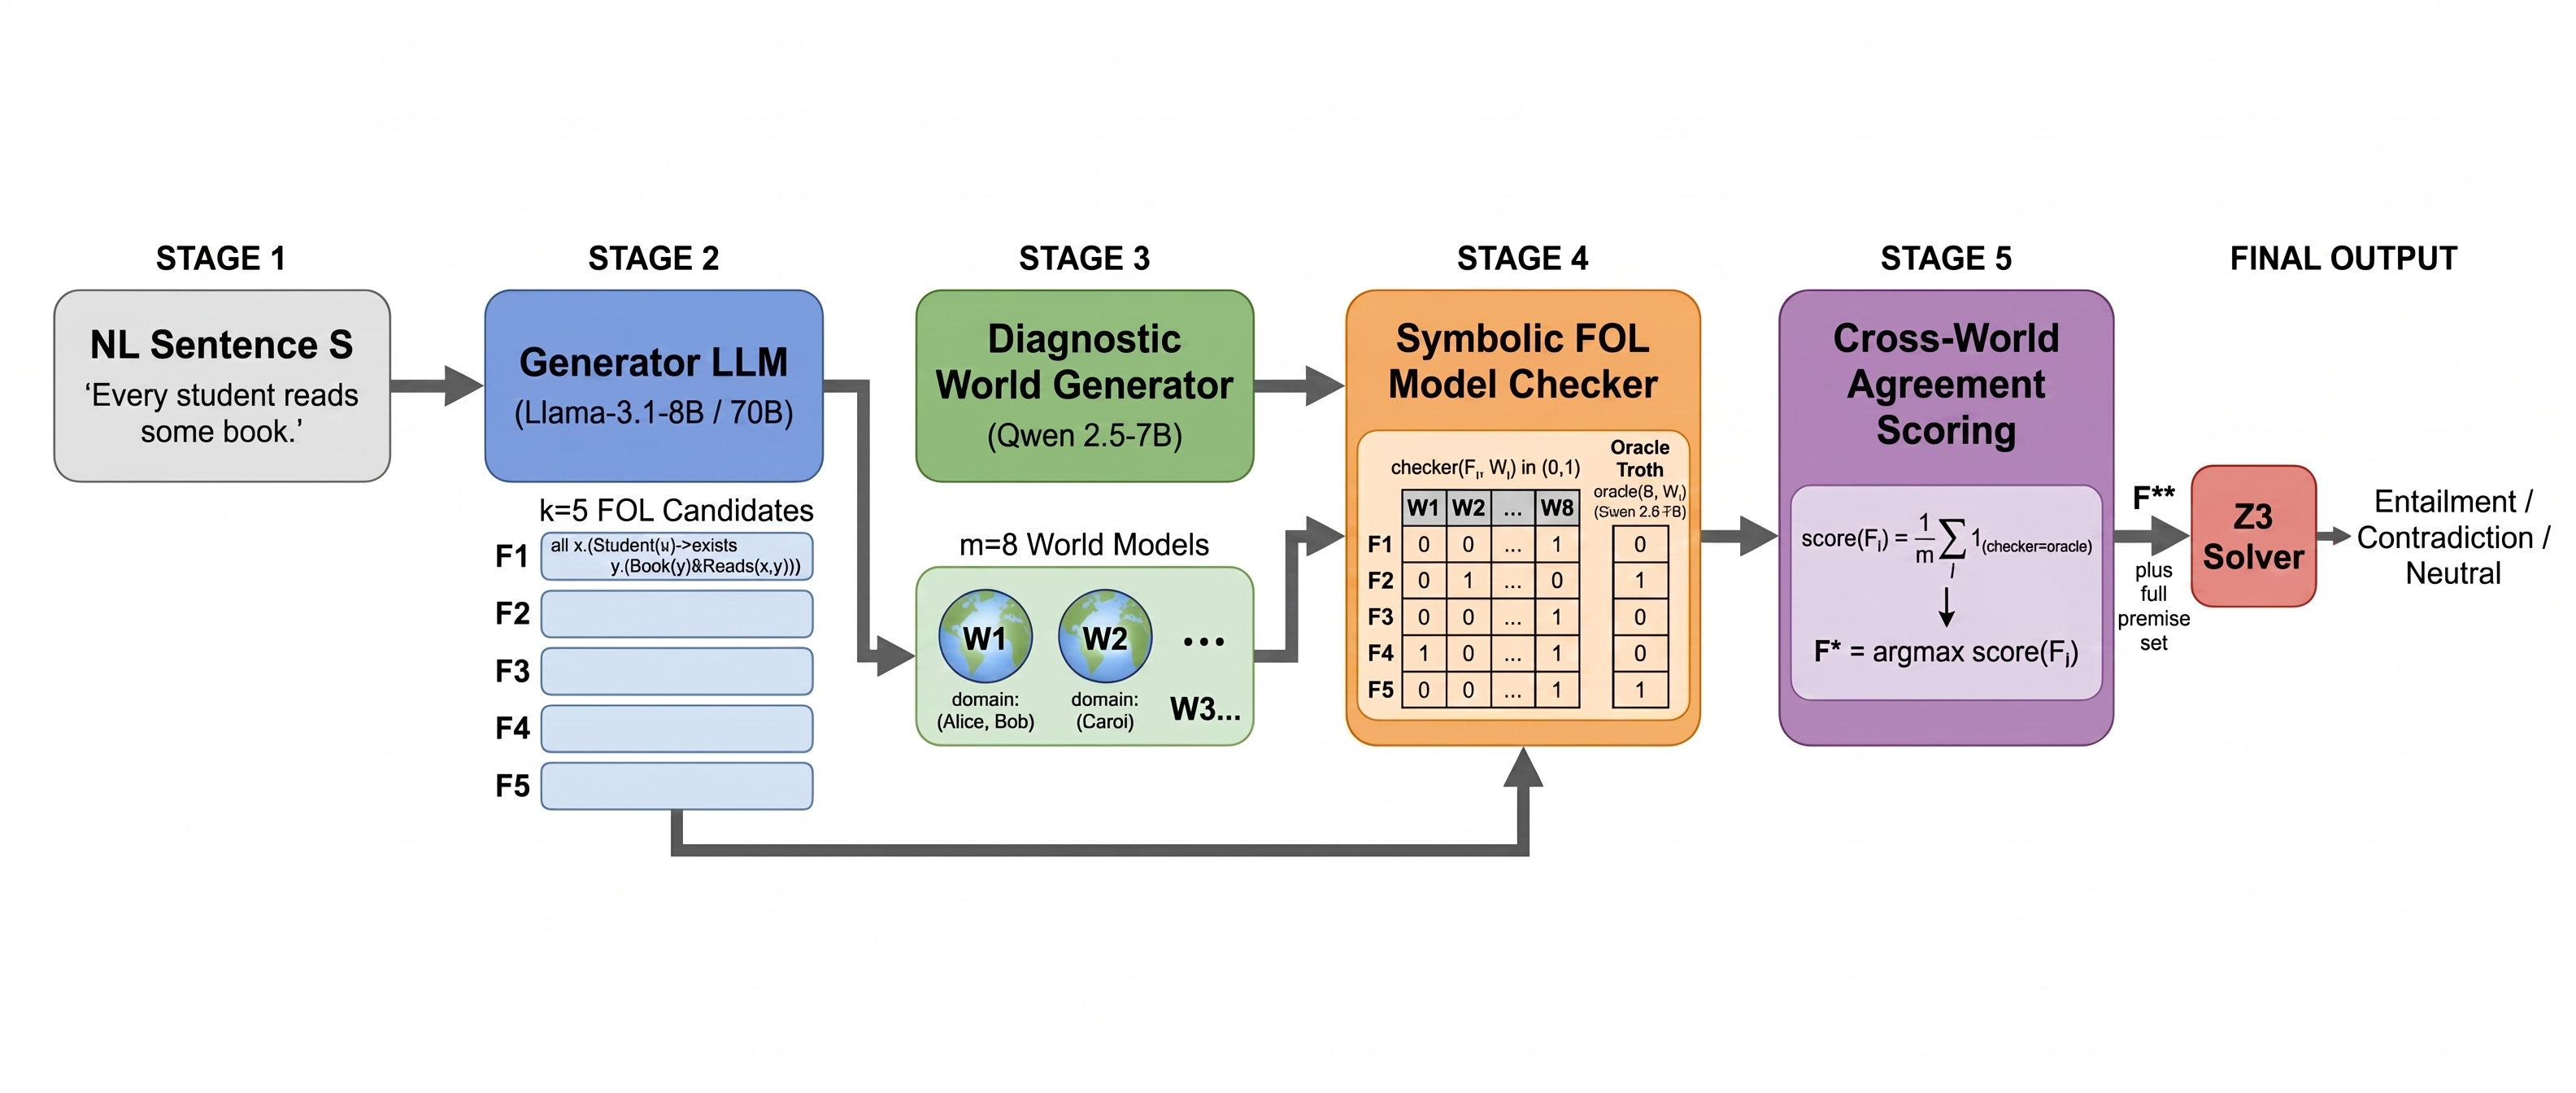
\includegraphics[width=\textwidth,height=0.45\textheight,keepaspectratio]{figures/fig_pipeline_v0.jpg}
  \caption{The Heterogeneous-Oracle World-Probing (HOWP) pipeline for annotation-free NL-to-FOL candidate selection. Given an NL sentence, the generator produces $k{=}5$ FOL candidates. For each candidate, $m{=}8$ diagnostic worlds are generated by the oracle LLM (from a different model family), evaluated deterministically by the symbolic model checker, and scored by cross-world agreement with oracle truth judgments. The highest-scoring candidate is passed to Z3 for downstream inference.}
  \label{fig:pipeline}
\end{figure*}

Our contributions are:
\begin{itemize}
  \item \textbf{HOWP pipeline}: An end-to-end annotation-free world-probing system combining LLM-based world generation, a deterministic Python FOL model checker, and cross-world agreement scoring (\S\ref{sec:method}).
  \item \textbf{Two-regime analysis}: We demonstrate that beam recall (38\% on FOLIO with Llama-3.1-8B; 100\% on synthetic data with Llama-3.1-70B) is the primary determinant of whether selection mechanisms can have measurable impact (\S\ref{sec:experiments}).
  \item \textbf{Discriminative signal under failure}: Even when HOWP cannot improve accuracy due to the beam recall ceiling, the cross-world agreement score retains a statistically significant discriminative signal (AUC-ROC $= 0.660$, Kendall $\tau = 0.212$, $p = 0.0009$), confirming the mechanism's soundness (\S\ref{sec:exp1-signal}).
  \item \textbf{Oracle noise analysis}: On the synthetic benchmark with 100\% beam recall, direct oracle judgment (99\%) outperforms HOWP (93\%) because 33\% oracle noise introduces selection errors on sentences simple enough not to require world scaffolding (\S\ref{sec:exp2}).
  \item \textbf{Independence hypothesis refutation}: The same-model oracle numerically outperforms the heterogeneous oracle on FOLIO (24.5\% vs.\ 20.6\%), with all differences non-significant ($p = 0.77$), suggesting that syntax calibration dominates parametric independence at 7B scale (\S\ref{sec:exp1-results}).
\end{itemize}

%% ============================================================
\section{Related Work}
%% ============================================================

\paragraph{NL-to-FOL Generation.}
NL2LOGIC \citep{Putra2025} introduces AST-guided generation that decomposes FOL translation into recursive semantic parsing steps, achieving 99\% syntactic accuracy on FOLIO. Code4Logic \citep{Liu2025} frames NL-to-FOL as a progressive code-generation task. GCD \citep{Geng2023} enforces syntactic validity at the token level but cannot detect scope or negation errors that are syntactically valid. All three are \emph{generation} methods and do not address test-time candidate selection.

\paragraph{NL-to-FOL Evaluation.}
\citet{Brunello2026} propose a two-phase benchmarking protocol separating ontology extraction from logical translation, and critique the LE score for propositional misuse. Their protocol requires gold FOL annotations and a Z3 solver---a benchmarking tool, not a selection mechanism. \citet{Thatikonda2024} train a verifier model for binary FOL error detection but require annotated training data. HOWP requires no annotations at any stage.

\paragraph{Neuro-Symbolic Reasoning.}
LINC \citep{Olausson2023} combines LLMs with Prover9 for logical reasoning using NLTK logic module syntax. Logic-LM \citep{Pan2023} employs symbolic solvers for faithful reasoning. Both target the full reasoning pipeline rather than test-time candidate selection.

\paragraph{Execution-Guided Semantic Parsing.}
Selecting formal expressions by execution against an environment is standard in database semantic parsing \citep{Pasupat2015, Min2019}. In database settings, the world is a fixed database and execution is deterministic---no oracle is needed. HOWP generates synthetic worlds to probe semantic distinctions and requires an LLM oracle because NL truth in abstract worlds is not mechanically computable.

\paragraph{Self-Consistency.}
\citet{Wang2023} propose sampling $k$ reasoning chains and selecting by majority vote. We adapt this to NL-to-FOL as a baseline: cluster $k{=}5$ translations by character $n$-gram similarity and pick the largest-cluster centroid. Our statistical re-analysis shows that alpha-renaming bound variables before clustering changes the selected candidate in 0\% of FOLIO examples, confirming that the SC baseline is robust to variable naming artifacts.%
\footnote{Code: \url{https://github.com/AMGrobelnik/ai-invention-8ad782-beam-recall-as-the-binding-constraint-an/tree/main/round-2/evaluation-1}}

\paragraph{Ensemble Theory.}
\citet{Breiman2001} showed that ensemble diversity determines generalization. \citet{Lakshminarayanan2017} derive uncertainty estimation power from parameter-space independence in deep ensembles. Both results assume models with identical architecture trained from different initializations---a stronger independence condition than the cross-family 7B-parameter models we test. Our empirical results show this assumption does not transfer to cross-family model pairs at this scale.

%% ============================================================
\section{Method}
\label{sec:method}
%% ============================================================

\subsection{Problem Formulation}

Given an NL sentence $S$ (a premise or conclusion from FOLIO \citep{Han2022}), a candidate generator produces $k$ FOL candidate translations $\{F_1, \ldots, F_k\}$. The goal is to select the candidate $F^*$ with highest semantic faithfulness to $S$ without access to gold FOL annotations. Faithfulness is operationalized as \emph{downstream inference accuracy}: whether substituting $F^*$ into the full FOLIO problem (premise set + conclusion) and running Z3 \citep{deMoura2008} produces the correct entailment/contradiction/neutral verdict.

\subsection{Pipeline Overview}

HOWP proceeds in four phases illustrated in Figure~\ref{fig:pipeline}.

\textbf{Phase 0 --- Beam Recall Gate.} Before running the full pipeline, measure the oracle upper bound: generate $k{=}5$ candidates with the generator LLM and check whether \emph{any} candidate produces the correct Z3 verdict on the FOLIO problem. This bounds the maximum accuracy achievable by any selection strategy and gates whether the experiment should proceed.

\textbf{Phase 1 --- Oracle Calibration Pilot.} On hand-constructed (sentence, world, truth-value) triples spanning simple predication (A), explicit negation (B), and quantifier scope ambiguity (C), measure the oracle LLM's binary truth-judgment accuracy against human ground truth. This validates that the oracle provides a discriminative signal and calibrates expected noise in the main experiment.

\textbf{Phase 2 --- Main World-Probing Pipeline.} For each FOLIO example:
\begin{enumerate}
  \item Generate $k{=}5$ FOL candidate translations using the generator LLM with 5-shot prompting in NLTK logic module syntax.
  \item Apply syntactic pre-filter: exclude candidates where open-domain existential quantifiers without named witnesses would invalidate the closed-world assumption (0.5\% filter rate in FOLIO experiments).
  \item Generate $m{=}8$ \emph{diagnostic world models} using the oracle LLM: each world is a minimal finite structure over 3--7 explicitly named domain elements, with ground atoms chosen to discriminate between competing semantic interpretations of $S$.
  \item Evaluate each candidate $F_i$ in each world $W_j$ using the deterministic Python FOL model checker, yielding $\text{checker}(F_i, W_j) \in \{0,1\}$.
  \item Query the oracle for truth judgment $\text{oracle}(S, W_j) \in \{0,1\}$ for each world.
  \item Compute cross-world agreement:
  \[
    \text{score}(F_i) = \frac{1}{m}\sum_j \mathbf{1}\bigl[\text{checker}(F_i, W_j) = \text{oracle}(S, W_j)\bigr].
  \]
  \item Select $F^* = \arg\max_i \text{score}(F_i)$, breaking ties by generation order.
\end{enumerate}

\textbf{Phase 3 --- Baselines and Ablations.} All conditions evaluate via Z3-based downstream accuracy. Baselines: (i) \emph{top-1}: take the first generated candidate; (ii) \emph{self-consistency}: cluster $k{=}5$ translations by Jaccard character $n$-gram similarity, select centroid of largest cluster; (iii) \emph{direct-judge}: ask the oracle to select the best formula directly without world models. Ablations: (A) \emph{same-model oracle}: use the generator model for both generation and oracle judgment; (B) \emph{random worlds}: replace diagnostic world generation with randomly sampled ground-atom combinations; (C) $m{=}4$ worlds: reduce world count from 8 to 4.

\subsection{Symbolic FOL Model Checker}

The deterministic model checker implements a recursive evaluator over finite named worlds. A world is represented as \texttt{\{'domain': list[str], 'atoms': dict[str, bool]\}}. Quantifiers iterate over explicitly listed domain elements under the closed-world assumption: existential quantifiers check if any domain element satisfies the body; universal quantifiers check all elements. The checker handles NLTK logic module syntax (\texttt{all x. (P(x) -> Q(x))}, \texttt{exists x. (P(x) \& Q(x))}, negation \texttt{-}, conjunction \texttt{\&}) and runs in milliseconds for formulas with $\leq 3$ quantifiers over domains of $\leq 10$ entities. Z3 \citep{deMoura2008} is used separately for final downstream inference evaluation.

\subsection{Implementation Details}

All LLM calls use the OpenRouter API. In Experiment~1 (FOLIO): generator is \texttt{meta-llama/llama-3.1-8b-instruct} \citep{Dubey2024}; oracle is \texttt{qwen/qwen-2.5-7b-instruct} \citep{Qwen2025}. In Experiment~2 (synthetic): generator is \texttt{meta-llama/llama-3.1-70b-instruct}; oracle is \texttt{qwen/qwen-2.5-7b-instruct}. Both experiments use a hard cost-halt at \$9.00; Experiment~1 cost \$0.43, Experiment~2 cost \$0.08.

%% ============================================================
\section{Experiments}
\label{sec:experiments}
%% ============================================================

\subsection{Experiment 1: FOLIO Benchmark}

\subsubsection{Dataset and Setup}

We use the FOLIO benchmark \citep{Han2022},%
\footnote{Code: \url{https://github.com/AMGrobelnik/ai-invention-8ad782-beam-recall-as-the-binding-constraint-an/tree/main/round-1/dataset-1}}
a 1,430-example NL reasoning dataset with gold FOL annotations. We evaluate on a stratified sample of 204 validation examples balanced across entailment/contradiction/neutral labels (72/63/69) and quantifier complexity tiers (0/1/2+ quantifiers). The beam recall analysis uses 50 held-out validation examples; the oracle calibration pilot uses 30 hand-constructed sentence-world pairs.

\subsubsection{Phase 0: Beam Recall Analysis}

On 50 FOLIO examples, Llama-3.1-8B with $k{=}5$ candidates achieves \textbf{38\% beam recall}---at least one of the five candidates produces the correct Z3 verdict for only 38\% of examples. This violates the pre-specified $\geq 60\%$ gate. We proceed with the experiment because the 38\% ceiling is itself a primary empirical finding: it quantifies the maximum accuracy achievable by \emph{any} selection strategy over this generator-benchmark pair, and understanding how existing selection mechanisms perform within a constrained beam is informative even when the gate fails.

\subsubsection{Phase 1: Oracle Calibration}

On 30 (sentence, world, truth-value) triples, Qwen2.5-7B-Instruct achieves \textbf{76.7\% agreement with human ground truth}, passing the $\geq 72\%$ gate. Performance is uneven across categories: most accurate on simple predication (category A) and least accurate on quantifier scope (category C). We emphasize that these triples are hand-constructed by the paper authors and may not reflect oracle accuracy on the LLM-generated worlds in Phase 2. A complementary in-distribution calibration is reported in Experiment 2 (\S\ref{sec:exp2}).

\subsubsection{Main Results}
\label{sec:exp1-results}

Table~\ref{tab:folio} summarizes accuracy and 95\% bootstrap confidence intervals for all seven conditions on 204 FOLIO examples. Figure~\ref{fig:results} plots the forest diagram.

\begin{table}[!htbp]
\centering
\caption{FOLIO benchmark results (n=204, Llama-3.1-8B generator). All pairwise McNemar tests are non-significant after Benjamini-Hochberg correction ($p_{\text{adj}} = 0.77$ for all pairs; Cohen's $h \leq 0.14$).}
\label{tab:folio}
\begin{tabular}{lccc}
\toprule
\textbf{Condition} & \textbf{Accuracy} & \textbf{95\% CI} & \textbf{Type} \\
\midrule
Same-Model Oracle   & 24.5\% & [18.6\%, 30.4\%] & Ablation \\
$m{=}4$ Worlds      & 23.5\% & [18.1\%, 29.4\%] & Ablation \\
Random Worlds       & 23.0\% & [17.6\%, 28.9\%] & Ablation \\
Direct Judge        & 20.1\% & [14.7\%, 25.5\%] & Baseline \\
Self-Consistency    & 20.6\% & [15.2\%, 26.5\%] & Baseline \\
\textbf{HOWP (Hetero-Oracle)} & \textbf{20.6\%} & [15.2\%, 26.5\%] & \textbf{Main} \\
Top-1 Generation    & 19.6\% & [14.2\%, 25.0\%] & Baseline \\
\midrule
Beam Recall Ceiling & 38.0\% & -- & Upper bound \\
\bottomrule
\end{tabular}
\end{table}

\begin{figure*}[!t]
  \centering
  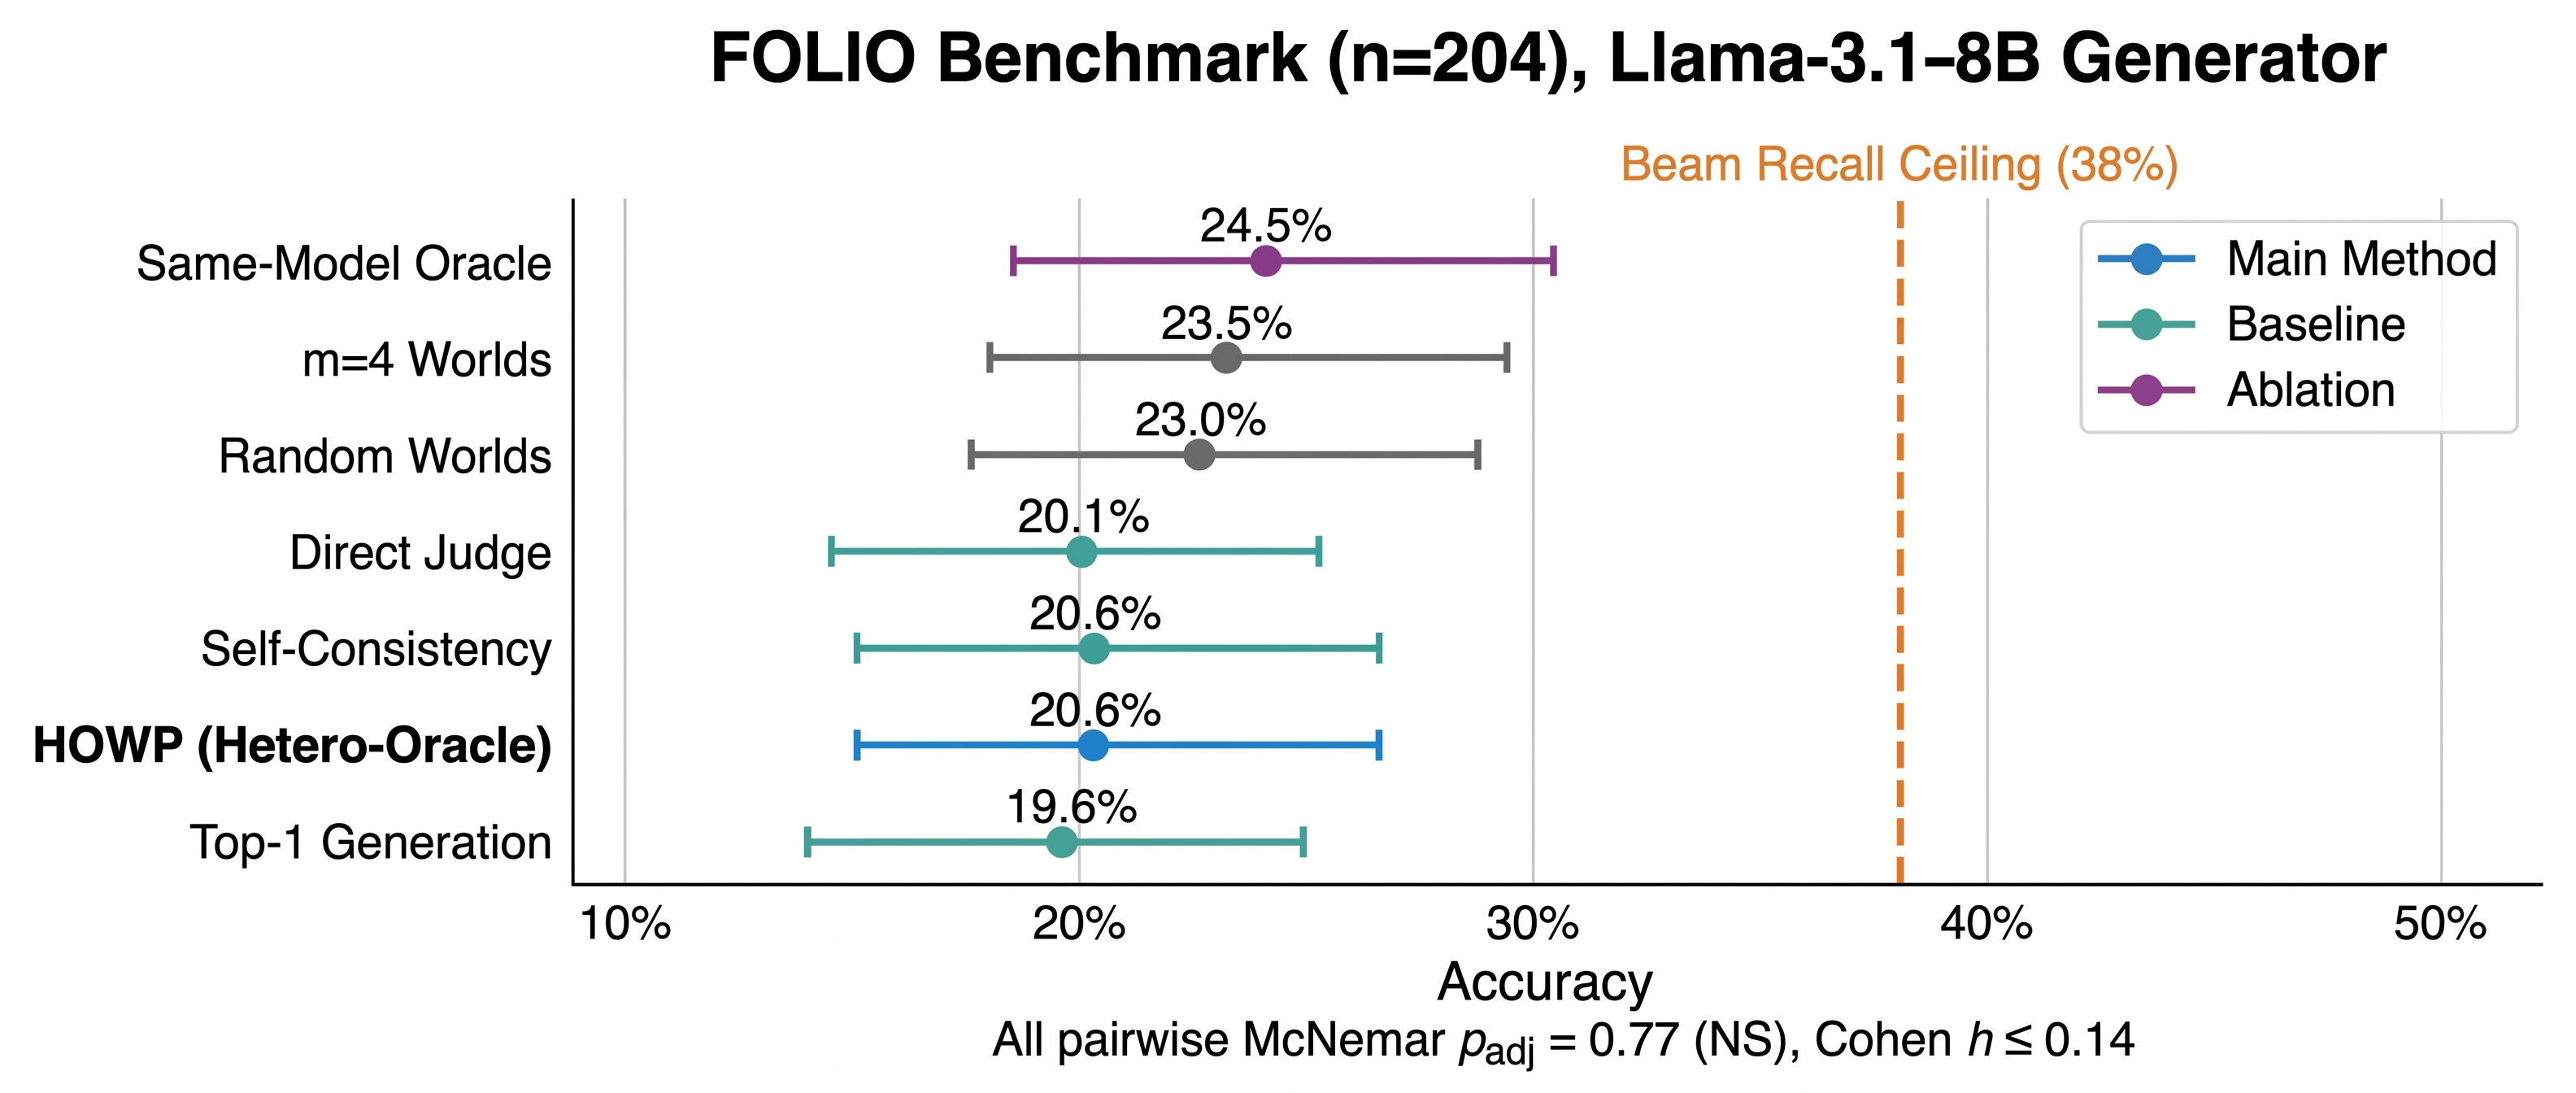
\includegraphics[width=\textwidth,height=0.45\textheight,keepaspectratio]{figures/fig_results_v0.jpg}
  \caption{Downstream inference accuracy on 204 FOLIO validation examples for all seven conditions, with 95\% bootstrap confidence intervals (10,000 resamples). All pairwise McNemar tests are non-significant after Benjamini-Hochberg correction ($p_{\text{adj}} = 0.77$ for all pairs; Cohen's $h \leq 0.14$). The 38\% beam recall ceiling (dashed orange line) sets the maximum achievable accuracy for any selection strategy.}
  \label{fig:results}
\end{figure*}

The heterogeneous-oracle main method achieves \textbf{20.6\%} accuracy (95\% CI: [15.2\%, 26.5\%]). All pairwise differences are non-significant after Benjamini-Hochberg correction (all $p_{\text{adj}} = 0.77$; Cohen's $h \leq 0.14$). The same-model oracle ablation achieves the numerically highest value at \textbf{24.5\%} [18.6\%, 30.4\%], but the McNemar test for heterogeneous vs.\ same-model oracle yields $\chi^2 = 0.67$, $p_{\text{adj}} = 0.77$, $h = -0.058$---a negligible effect. No condition is distinguishable from any other at $n{=}204$.

Label-stratified accuracy shows large within-condition variance: Uncertain 36.2\%, Entailment 13.9\%, Contradiction 11.1\%. Importantly, the Uncertain-class accuracy is entirely artifactual: among 69 gold-Uncertain examples, the main method predicts `Uncertain' for 25 (coincidence hits via empty-string parse failure defaulting to Uncertain) and outputs an empty string for 41; 100\% of the Uncertain-class correct predictions arise from coincidence rather than genuine logical inference. Empty-string rates across conditions range from 55\% to 65\%, reflecting the frequency with which Llama-3.1-8B generates FOL that the Z3 pipeline cannot parse.

\subsubsection{Discriminative Signal Analysis}
\label{sec:exp1-signal}

Despite uniform downstream accuracy, the cross-world agreement score retains a statistically significant discriminative signal. AUC-ROC for predicting per-example correctness from the maximum world agreement score among the five candidates is \textbf{0.660}, and Kendall $\tau = 0.212$ ($p = 0.0009$). The mean maximum world agreement score for correctly-solved examples is 0.857 vs.\ 0.742 for incorrectly-solved examples. This confirms that the HOWP mechanism produces a valid ranking signal---the selection failures at the accuracy level are not due to the mechanism being uninformative, but to the 38\% beam recall ceiling limiting the opportunity for any selection to matter.

The inter-model agreement analysis further clarifies: the heterogeneous and same-model oracles select the same candidate in 77.5\% of examples (158/204). When the same-model oracle is wrong, the heterogeneous oracle is correct only 5.8\% of the time---confirming that the two oracles largely fail and succeed on the same examples.

\subsection{Experiment 2: Synthetic Benchmark with High Beam Recall}
\label{sec:exp2}

\subsubsection{Motivation and Setup}

Experiment~1 cannot distinguish mechanism design from beam recall effects at 38\%. To isolate the mechanism, we construct a synthetic single-premise NLI benchmark%
\footnote{Code: \url{https://github.com/AMGrobelnik/ai-invention-8ad782-beam-recall-as-the-binding-constraint-an/tree/main/round-2/experiment-1}}
where beam recall is substantially higher. We use 175 examples (50 beam recall, 100 main, 25 oracle validation) with controlled FOL structure covering three label types: entailment (all X are Y + X(name) $\to$ Y(name)), contradiction (no X are Y + X(name) $\leftrightarrow \neg$Y(name)), and neutral (some X are Y $\not\to$ Y(name)). Gold FOL is in NLTK syntax for Z3 verification. We upgrade the generator to \textbf{Llama-3.1-70B} to ensure high beam recall.

\subsubsection{Beam Recall and Oracle Accuracy}

Beam recall with Llama-3.1-70B and $k{=}5$ candidates is \textbf{100\%}: for every example, at least one of the five candidates produces the correct Z3 verdict. The oracle calibration pilot on 25 in-distribution examples (LLM-generated worlds, not hand-constructed) yields \textbf{66.7\% oracle accuracy}---substantially lower than the 76.7\% accuracy on hand-constructed triples in Experiment~1, confirming that in-distribution world-probing is harder than the Phase~1 pilot suggested.

\subsubsection{Results}
\label{sec:exp2-results}

\begin{figure*}[!t]
  \centering
  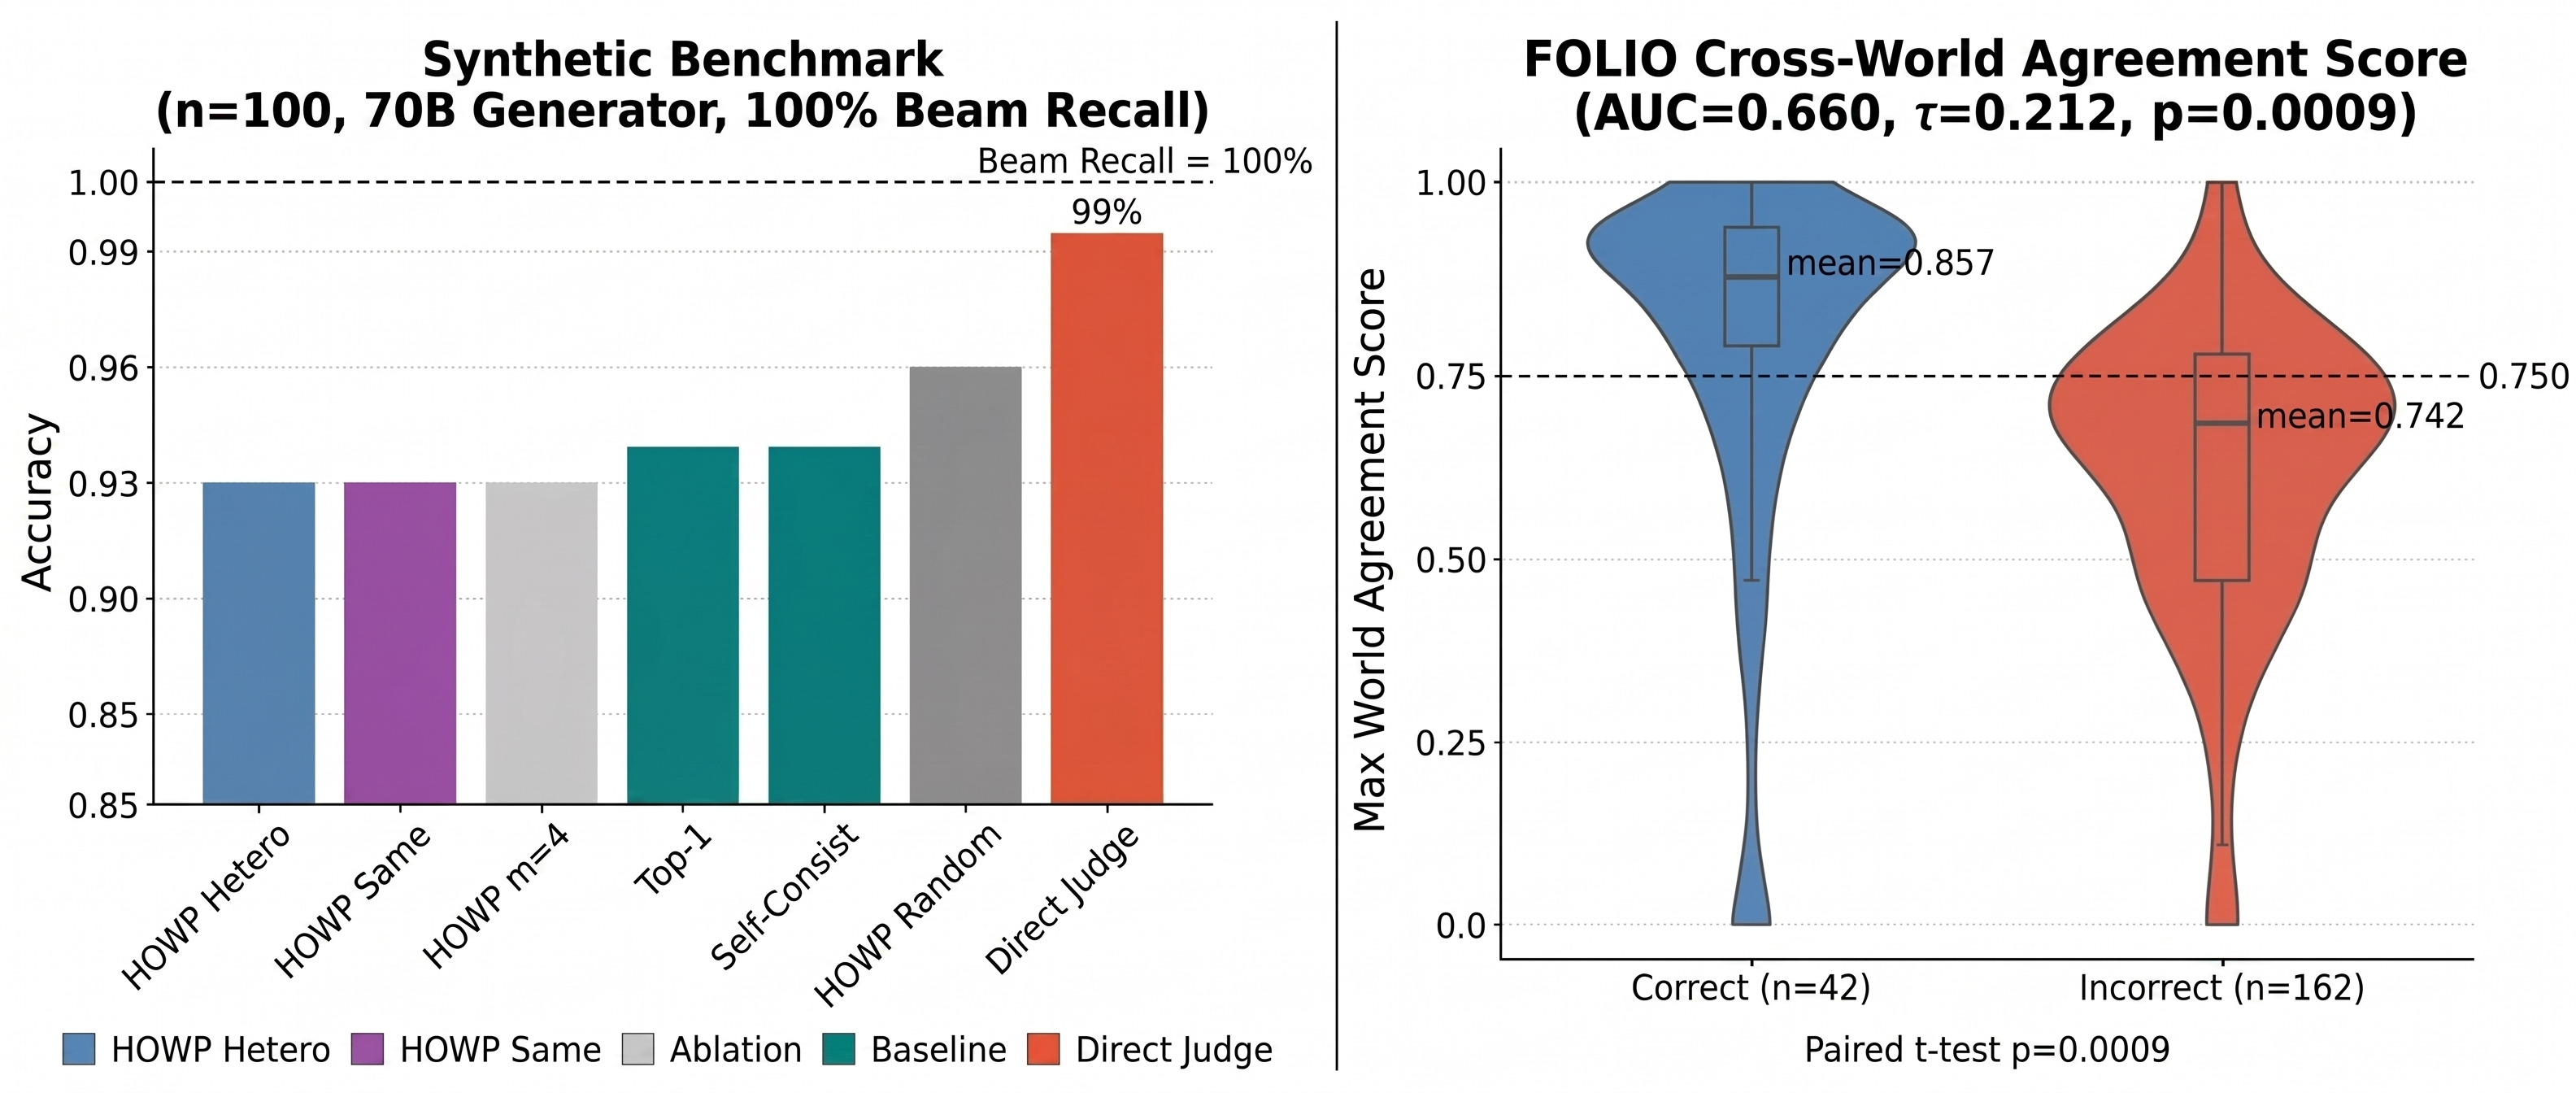
\includegraphics[width=\textwidth,height=0.45\textheight,keepaspectratio]{figures/fig_synthetic_v0.jpg}
  \caption{\textbf{Left:} Accuracy on the synthetic single-premise NLI benchmark (n=100, Llama-3.1-70B generator, 100\% beam recall). Direct oracle judgment (99\%) outperforms all HOWP variants (93\%) and baselines (94\%), because 33\% oracle noise hurts world-probing selection on simple sentences. \textbf{Right:} On FOLIO (n=204), the maximum cross-world agreement score among candidates has AUC-ROC $= 0.660$ and Kendall $\tau = 0.212$ ($p = 0.0009$) for predicting per-example correctness, confirming the mechanism's discriminative signal despite the beam recall ceiling.}
  \label{fig:synthetic}
\end{figure*}

With 100\% beam recall (Figure~\ref{fig:synthetic}):
\begin{itemize}
  \item HOWP heterogeneous oracle: \textbf{93\%} (93/100)
  \item HOWP same-model oracle: \textbf{93\%} (93/100)
  \item HOWP random worlds: \textbf{96\%} (96/100)
  \item HOWP $m{=}4$ worlds: \textbf{93\%} (93/100)
  \item Top-1 generation: \textbf{94\%} (94/100)
  \item Self-consistency: \textbf{94\%} (94/100)
  \item \textbf{Direct oracle judgment: 99\%} (99/100)
\end{itemize}

Several findings emerge. First, HOWP (93\%) does not outperform top-1 generation (94\%) or self-consistency (94\%) even with 100\% beam recall, indicating that oracle noise (33\% error rate) introduces incorrect selections that offset the benefit of world-probing on these simple predicate-application sentences. Second, random worlds (96\%) match or exceed diagnostic worlds (93\%), suggesting that for simple sentence types the discriminative value of purpose-built worlds over random worlds is negligible. Third, direct oracle judgment (99\%) substantially outperforms all HOWP variants, because when the sentence is simple enough for the oracle to judge directly, the world-scaffolding step adds noise without proportionate benefit.

Note that all comparisons on $n{=}100$ examples are subject to high variance; the 6-percentage-point gap between direct-judge (99\%) and HOWP (93\%) corresponds to 6 examples and should be interpreted with appropriate uncertainty. The primary value of this experiment is establishing that beam recall alone does not guarantee HOWP gains---oracle quality and sentence complexity jointly determine whether world-probing adds value over direct judgment.

%% ============================================================
\section{Discussion}
%% ============================================================

\subsection{The Two-Regime Picture}

The two experiments paint a coherent picture of the conditions under which HOWP can succeed. In the low-beam-recall regime (FOLIO, 38\%), the binding constraint is generation quality: with fewer than 2 in 5 beams containing a correct candidate, even a perfect selection oracle cannot exceed 38\% accuracy, and the observed 19.6\%--24.5\% range is consistent with imperfect selection over a constrained beam. The cross-world agreement score's significant AUC (0.660) and Kendall $\tau$ (0.212) confirm the mechanism is not noise---it is simply under-powered against a hard ceiling.

In the high-beam-recall regime (synthetic, 100\%), the binding constraint shifts to oracle noise. The 66.7\% in-distribution oracle accuracy introduces approximately one incorrect judgment per three worlds. For simple predicate-application sentences where the oracle could judge directly at 99\% accuracy, the world-scaffolding layer adds processing that amplifies oracle errors without providing discriminative benefit beyond direct judgment.

These two regimes together define the operating window for HOWP: it requires (a) a generator with beam recall sufficiently high that correct candidates are frequently available, and (b) sentences complex enough (multi-quantifier, ambiguous scope) that direct oracle judgment is unreliable but world-probing disambiguates. Neither condition was met in our experiments: FOLIO had insufficient beam recall, and the synthetic benchmark had insufficient sentence complexity.

\subsection{Why the Heterogeneity Hypothesis Did Not Hold}

The ensemble-theory motivation for oracle heterogeneity assumes that intra-model self-consistency bias is the dominant source of error, and that parametric independence between generator and oracle breaks this bias. Our results suggest an alternative: when candidate formulas are expressed in syntax learned by model A, model B's judgments may be less calibrated to that syntax than model A's own judgments---even accounting for self-consistency concerns.

For Llama-3.1-8B generating NLTK-syntax FOL, Qwen2.5-7B-Instruct (trained on different corpora and syntax conventions) interprets scope operators and negation slightly differently. The same-model oracle's numerical advantage (24.5\% vs.\ 20.6\%, though non-significant) is consistent with Llama's judgments about its own generated formulas being better calibrated to the NLTK syntax it produces.

The ensemble-theory argument requires roughly equal cross-task calibration across oracle models. Our evidence suggests this does not hold for cross-family 7B-parameter models on NLTK-syntax FOL. The independence benefit may require larger models with more uniform calibration, or oracle models explicitly fine-tuned on the generator's output syntax.

\subsection{Limitations}

\begin{enumerate}
  \item \textbf{Scale}: Both generator (8B for FOLIO) and oracle (7B) are small models. The heterogeneity benefit may emerge at scales where cross-family calibration is more uniform.
  \item \textbf{Benchmark mismatch}: FOLIO's multi-hop reasoning chains (3--8 premises per problem) were designed to evaluate full-system reasoning, not per-sentence FOL translation. Per-sentence world-probing does not capture inter-premise consistency, which limits its advantage.
  \item \textbf{Oracle calibration gap}: The 10-percentage-point gap between hand-constructed pilot accuracy (76.7\%) and in-distribution accuracy (66.7\%) indicates that oracle quality is harder to validate than the Phase~1 protocol suggests. In-distribution calibration should be the primary gate.
  \item \textbf{Synthetic benchmark simplicity}: The controlled benchmark's simple predicate-application structure does not probe the scope ambiguities and negation interactions where HOWP's world-probing is most motivated. A benchmark with explicit quantifier-scope variation and high beam recall remains to be evaluated.
  \item \textbf{Parse failure rate}: Empty-string rates of 55--65\% on FOLIO indicate that a large fraction of Llama-3.1-8B's FOL outputs cannot be parsed by Z3. Cleaning the generator's output syntax would improve the effective beam recall substantially.
\end{enumerate}

%% ============================================================
\section{Conclusion}
%% ============================================================

We presented HOWP, an annotation-free world-probing pipeline for NL-to-FOL candidate selection, and evaluated it under two qualitatively different experimental regimes. On FOLIO with Llama-3.1-8B (38\% beam recall), no selection method---including HOWP, top-1, self-consistency, and three ablations---is distinguishable (all McNemar $p_{\text{adj}} = 0.77$), yet the cross-world agreement score retains a significant discriminative signal (AUC $= 0.660$, $\tau = 0.212$, $p = 0.0009$). On a synthetic benchmark with Llama-3.1-70B (100\% beam recall), direct oracle judgment (99\%) outperforms HOWP (93\%) because 33\% oracle noise hurts selection when sentences are simple enough for direct judgment. The same-model oracle ablation numerically exceeds the heterogeneous design on FOLIO (24.5\% vs.\ 20.6\%, non-significant), suggesting syntax calibration outweighs parametric independence at 7B scale.

These results establish beam recall as the primary bottleneck: HOWP's world-probing mechanism is sound but requires a generator achieving $\geq 60\%$ beam recall before selection effects can exceed statistical noise. Future work should:
\begin{itemize}
  \item Evaluate HOWP with a generator that achieves $\geq 60\%$ beam recall on FOLIO (e.g., Llama-3.1-70B or GPT-4o).
  \item Construct a benchmark combining high beam recall with complex quantifier-scope sentences, to activate HOWP's discriminative advantage in the regime where direct oracle judgment is unreliable.
  \item Fine-tune oracle models on the generator's output syntax before assuming calibration equality.
  \item Investigate premise-set-level selection that maintains inter-sentence consistency rather than selecting each sentence independently.
\end{itemize}

The HOWP infrastructure---world generator, symbolic model checker, cross-world scoring---constitutes a reusable foundation for annotation-free semantic faithfulness evaluation once the generation and oracle quality conditions are met.

\bibliography{references}
\bibliographystyle{plainnat}

\end{document}
